Recent literature shows that model-based, model-free and hybrid control strategies have been used to control soft robots. However, the developed model-based control algorithms predominantly used kinematic descriptions of the robots, rather than dynamical models. Although there are studies that use dynamical models  \cite{falkenhahn2016dynamic}, \cite{della2020model}, and \cite{kapadia2011task}, a lot of research in this field is left undone. With this master thesis we aim to find an model-based control strategy that will generally result in higher tracking performance of the soft robot. Hence, the research objective follows:



\textit{Develop a model-based control strategy for a pneumatically actuated, hyper-redundant soft robot (Figure \ref{fig:sorotoki}) to perform a reference tracking problem}




\begin{figure}[H]
    \centering
    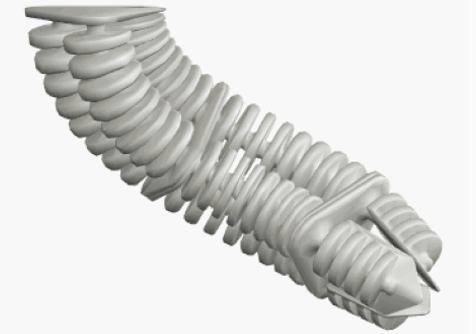
\includegraphics{Figures/sorotoki1.png}
    \caption{Computer image of the soft robot used in this project.}
    \label{fig:sorotoki}
\end{figure}


To effectively answer the research objective we might consider previous research on under-actuated classic robots, and try to apply these methods to soft robots.

Sliding mode control (SMC) can be used to control under-actuated systems. SMC can be an effective tool in controller design, as it is insensitive to model errors and external disturbances. Reason for this is that the behaviour on the sliding mode depends only on the defined switching surface, not the structural properties of the system \cite{liu2013survey}. In \cite{xu2008sliding} a theory is presented to globally stabilize all degrees of freedom, including the non-linearly coupled, indirectly actuated degrees of freedom for a system in cascaded form. By defining a sliding surface, the un-actuated degrees of freedom can be stabilized, and the actuated degrees of freedom controlled.

In \cite{liu2013survey}, the theory of fuzzy control for under-actuated systems is presented. This control strategy is used to mimic human logic and can therefore deal with imprecise, uncertain or qualitative decision-making situations. Although it is considered a non-mathematical control strategy to control system where model making is difficult \cite{michels2007fuzzy}, plenty of model-based fuzzy controllers have been designed e.g. \cite{begovich2002takagi} and \cite{tao2008design}. 

Instead of SMC and fuzzy control, backstepping \cite{khalil2002nonlinear} can be used to control the system. This control approach transforms the system to a new recursive form, where a sequence of "virtual" systems is created. By selecting the "virtual" input, the system can be made globally asymptotically stable. Backstepping has been previously used for under-actuated systems such as \cite{madani2006backstepping}.

In \cite{spong1994linear}, non-linear partial feedback linearization is discussed. The mechanical system is described in generalized coordinates, and divided in actuated and un-actuated degrees of freedom. The theory presented, shows that under "strong inertial coupling" the actuated joints can linearize the un-actuated degrees of freedom. 

Energy based control \cite{spong1996energy} is another approach to control the under-actuated mechanical system. In essence, nonlinear partial feedback linearization is used, together with energy shaping. For the system an energy function is determined, enabling to calculate the total energy at a given point. By using multiple controllers and switching between those, under-actuated systems can stabilize around their desired end-effector position. The theory and application of energy based control for Euler-Lagrange systems has been captured very well in \cite{ortega2013passivity}.


Although the aforementioned control approaches are only applied to classic rigid mechanical systems, they could be relevant to a broader field of under actuated systems, such as infinite dimensional soft robots. Since a model-based controller is desired, the focus will initially be at designing an energy-based controller.



